\section{Stawianie budowli (Zofia Sosińska)}\label{chap:omd}
Jedną z kluczowych mechanik gier z gatunku RTS jest budowanie budynków. Funkcjonalność pozwala graczowi 
na podejmowanie strategicznych decyzji w zależności od potrzeb i możliwości budowli. Funkcje pełnione 
przez budynek mogą być bardzo różnorodne. W niektórych przypadkach ich zadaniem jest produkcja surowców, czy leczenie
jednostek, ale są i takie, które skupiają się na wspieraniu gracza w obliczu zagrożenia. Mogą to być fortyfikacje opóźniające natarcie,
bądź chociażby machiny wojenne towarzyszące ofensywie.

Orcs must die! to strategiczna gra akcji stworzona i wydana przez studio Robot Entertainment. Zadaniem gracza jest wcielenie się
w jednego z Wojennych Magów i mordowanie nadciągających grup orków za pomocą różnorodnych broni i mechanizmów, które może postawić.
W przejrzysty sposób zostało rozwiązane samo wyświetlenie dostępnych do zbudowania pułapek. Na dole ekranu pokazują się wizerunki mechanizmów,
które może postawić oraz informacja o ich cenie. Naciskając odpowiedni numer na klawiaturze, gracz wybiera, co chce zbudować. Po zatwierdzeniu lewym przyciskiem myszki,
budynek pojawia się w zaznaczonym miejscu. Od tego momentu pułapka będzie pomocą dla głównej postaci podczas zwarcia z przeciwnikami.
Jego ograniczeniem w stawianiu mechanizmów są jego fundusze, dlatego gracz musi przemysleć, co kupić oraz gdzie najoptymalniej będzie to postawić.

\begin{figure}[h!tbp]
    \centering
    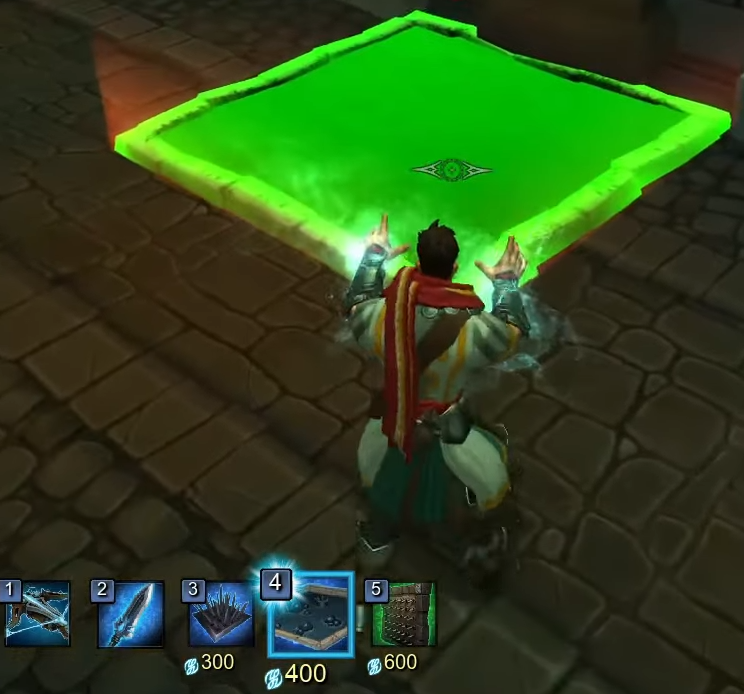
\includegraphics[width=0.9\textwidth]{images/ui/buoildingsOrcs.png}
    \caption{Wyświetlenie dostępnych pułapek w Orcs must die!}\label{fig:Orcs}
\end{figure}